%!TEX program = xelate
%%%%%%%%%%%%%%%%%%%%%%%%%%%%%%%%%%%%%%%%%
% Modified By Orcuslc, 2016-9-21
% Modified for Assignments
% http://github.com/orcuslc
%
% Wilson Resume/CV
% Structure Specification File
% Version 1.0 (22/1/2015)
%
% This file has been downloaded from:
% http://www.LaTeXTemplates.com
%
% License:
% CC BY-NC-SA 3.0 (http://creativecommons.org/licenses/by-nc-sa/3.0/)
%
%%%%%%%%%%%%%%%%%%%%%%%%%%%%%%%%%%%%%%%%%

%----------------------------------------------------------------------------------------
%	PACKAGES AND OTHER DOCUMENT CONFIGURATIONS
%----------------------------------------------------------------------------------------
\documentclass[10pt]{article}

\usepackage{listings}
\usepackage{xcolor}
\usepackage{amsmath,amsthm,amssymb}
\usepackage{epstopdf}
\usepackage{graphicx}
\usepackage{clrscode3e}

\DeclareGraphicsExtensions{.eps,.ps,.jpg,.bmp}


\usepackage[a4paper, hmargin=25mm, vmargin=30mm, top=20mm]{geometry} % Use A4 paper and set margins

\usepackage{fancyhdr} % Customize the header and footer

\usepackage{lastpage} % Required for calculating the number of pages in the document

\usepackage{hyperref} % Colors for links, text and headings

\setcounter{secnumdepth}{0} % Suppress section numbering

%\usepackage[proportional,scaled=1.064]{erewhon} % Use the Erewhon font
%\usepackage[erewhon,vvarbb,bigdelims]{newtxmath} % Use the Erewhon font
\usepackage[utf8]{inputenc} % Required for inputting international characters
\usepackage[T1]{fontenc} % Output font encoding for international characters

\usepackage{fontspec} % Required for specification of custom fonts
\setmainfont[Path = ./fonts/,
Extension = .otf,
BoldFont = Erewhon-Bold,
ItalicFont = Erewhon-Italic,
BoldItalicFont = Erewhon-BoldItalic,
SmallCapsFeatures = {Letters = SmallCaps}
]{Erewhon-Regular}

\usepackage{color} % Required for custom colors
\definecolor{slateblue}{rgb}{0.17,0.22,0.34}

\usepackage{sectsty} % Allows customization of titles
\sectionfont{\color{slateblue}} % Color section titles

\fancypagestyle{plain}{\fancyhf{}\cfoot{\thepage\ of \pageref{LastPage}}} % Define a custom page style
\pagestyle{plain} % Use the custom page style through the document
\renewcommand{\headrulewidth}{0pt} % Disable the default header rule
\renewcommand{\footrulewidth}{0pt} % Disable the default footer rule

\setlength\parindent{0pt} % Stop paragraph indentation

% Non-indenting itemize
\newenvironment{itemize-noindent}
{\setlength{\leftmargini}{0em}\begin{itemize}}
{\end{itemize}}

% Text width for tabbing environments
\newlength{\smallertextwidth}
\setlength{\smallertextwidth}{\textwidth}
\addtolength{\smallertextwidth}{-2cm}

\newcommand{\sqbullet}{~\vrule height .8ex width .6ex depth -.05ex} % Custom square bullet point 


\newcommand{\tbf}[1]{\textbf{#1}}
\newcommand{\tit}[1]{\textit{#1}}
\newcommand{\mbb}[1]{\mathbb{#1}}
\newcommand{\blue}[1]{\color{blue}{#1}}
\newcommand{\red}[1]{\color{red}{#1}}
\newcommand{\sblue}[1]{\color{slateblue}{#1}}
\newcommand{\n}{\\[5pt]}
\newcommand{\tr}{^\top}
\newcommand{\vt}[1]{
\Vert #1 \Vert
}
\newcommand{\bra}[5]{
#1=\left\{
\begin{aligned}
#2 ,&\quad #4 \\
#3 ,&\quad #5
\end{aligned}
\right.
}

\renewcommand{\title}[2] {
{\Huge{\color{slateblue}\textbf{#1}}}
\hfill
\LARGE{\color{slateblue}\textbf{#2}} \\[10pt]
\large{\color{slateblue}\textbf{Chuan Lu, 13300180056, chuanlu13@fudan.edu.cn}} \\[1mm]
\rule{\textwidth}{0.5mm}
}

\newcommand{\problem}[2] {
\vspace{20pt}
\LARGE{\color{slateblue}\textbf{Problem #1.}}
\vspace{2mm}
#2 \\[10pt]
}

\renewcommand{\proof}[2] {
\large{\color{slateblue}\textit{\textbf{#1.}}}
#2 \qed \\[3mm]
}

\newcommand{\solution}[2] {
\large{\color{slateblue}\textit{\textbf{#1.}}}
#2 \\[3mm]
}


\newcommand{\algorithm}[2] {
\begin{codebox}
\Procname{$\proc{Algorithm #1}$}
#2
\end{codebox}
}

\newcommand{\refgroup}[1] {
\LARGE{\color{slateblue}\textbf{Reference}} 
\begin{tabbing}
\hspace{5mm} \= \kill
#1
\end{tabbing}
}

\newcommand{\reference}[1] {
\sqbullet \ \  \large{#1} \\
}
% \newcommand{\solution}[2] {
% \LARGE{\color{slateblue}\textit{#1}}
% \ #2 \qed
% }

% \newenvironment{problem}[2][Problem]{\begin{trivlist}
% \item[\hskip \labelsep {\bfseries #1}\hskip \labelsep {\bfseries #2.}]}{\end{trivlist}}
\usepackage{epstopdf}
\usepackage{graphics}
\usepackage{subfig}
\usepackage{listings}
\lstset{
  breaklines=true,
  xleftmargin=25pt,
  xrightmargin=25pt,
  aboveskip=0pt,
  belowskip=10pt,
  basicstyle=\ttfamily,
  showstringspaces=false,
  frame=ltrb,
  tabsize=4,
  numbers=left,
  numberstyle=\small,
  numbersep=8pt,
  morekeywords={*, factorial, sum, erlang},
  keywordstyle=\color{blue!70}, commentstyle=\color{red!50!green!50!blue!50},
}
\DeclareGraphicsExtensions{.eps,.ps,.jpg,.bmp}

\begin{document}

\title{Numerical Analysis \\ Assignment 4}
\date{\today}
\author{Chuan Lu}

\maketitle

\problem{1}{Problem 2.2, Page 118}
\solution{Solution}{
The code of the three schemes are as follows.
}
\lstinputlisting[language = MATLAB]{bisection.m}
\lstinputlisting[language = MATLAB]{newton.m}
\lstinputlisting[language = MATLAB]{secant.m}
\lstinputlisting[language = MATLAB]{main.m}
\solution{Result}{
The result of output are as follows, and in each result there are three columns, index, value, error respectively.
}
\begin{lstlisting}[language = MATLAB]
>> main
                   0  -0.500000000000000   0.500000000000000
   1.000000000000000  -0.250000000000000   0.250000000000000
   2.000000000000000  -0.375000000000000   0.125000000000000
   3.000000000000000  -0.437500000000000   0.062500000000000
   4.000000000000000  -0.468750000000000   0.031250000000000
   5.000000000000000  -0.453125000000000   0.015625000000000
   6.000000000000000  -0.460937500000000   0.007812500000000
   7.000000000000000  -0.457031250000000   0.003906250000000
   8.000000000000000  -0.458984375000000   0.001953125000000
   9.000000000000000  -0.458007812500000   0.000976562500000
  10.000000000000000  -0.458496093750000   0.000488281250000
  11.000000000000000  -0.458740234375000   0.000244140625000
  12.000000000000000  -0.458862304687500   0.000122070312500
  13.000000000000000  -0.458923339843750   0.000061035156250
  14.000000000000000  -0.458953857421875   0.000030517578125
  15.000000000000000  -0.458969116210938   0.000015258789063
  16.000000000000000  -0.458961486816406   0.000007629394531
  17.000000000000000  -0.458965301513672   0.000003814697266
  18.000000000000000  -0.458963394165039   0.000001907348633
  19.000000000000000  -0.458962440490723   0.000000953674316

                   0  -0.500000000000000   0.500000000000000
   1.000000000000000  -0.460219570045525   0.039780429954475
   2.000000000000000  -0.458963518356852   0.001256051688672
   3.000000000000000  -0.458962267538189   0.000001250818663
   4.000000000000000  -0.458962267536949   0.000000000001240

                   0  -1.000000000000000   1.000000000000000
   1.000000000000000                   0   1.000000000000000
   2.000000000000000  -0.275321257596836   0.275321257596836
   3.000000000000000  -0.588196207258892   0.312874949662057
   4.000000000000000  -0.439364813249275   0.148831394009618
   5.000000000000000  -0.457108107412876   0.017743294163601
   6.000000000000000  -0.458991546782558   0.001883439369682
   7.000000000000000  -0.458962224440445   0.000029322342112
   8.000000000000000  -0.458962267535948   0.000000043095503
   9.000000000000000  -0.458962267536949   0.000000000001000

                   0   0.785398163397448   0.785398163397448
   1.000000000000000   1.178097245096172   0.392699081698724
   2.000000000000000   0.981747704246810   0.196349540849362
   3.000000000000000   1.079922474671491   0.098174770424681
   4.000000000000000   1.129009859883832   0.049087385212341
   5.000000000000000   1.104466167277661   0.024543692606170
   6.000000000000000   1.116738013580747   0.012271846303085
   7.000000000000000   1.122873936732289   0.006135923151543
   8.000000000000000   1.125941898308061   0.003067961575771
   9.000000000000000   1.127475879095946   0.001533980787886
  10.000000000000000   1.128242869489889   0.000766990393943
  11.000000000000000   1.128626364686860   0.000383495196971
  12.000000000000000   1.128434617088375   0.000191747598486
  13.000000000000000   1.128338743289132   0.000095873799243
  14.000000000000000   1.128386680188753   0.000047936899622
  15.000000000000000   1.128410648638564   0.000023968449811
  16.000000000000000   1.128422632863469   0.000011984224906
  17.000000000000000   1.128428624975922   0.000005992112453
  18.000000000000000   1.128425628919696   0.000002996056226
  19.000000000000000   1.128424130891582   0.000001498028113
  20.000000000000000   1.128424879905639   0.000000749014057

                   0   0.500000000000000   0.500000000000000
   1.000000000000000   1.167298749806364   0.667298749806364
   2.000000000000000   1.128496956086359   0.038801793720005
   3.000000000000000   1.128425093253079   0.000071862833280
   4.000000000000000   1.128425092992225   0.000000000260854

                   0                   0                   0
   1.000000000000000   1.000000000000000   1.000000000000000
   2.000000000000000   1.142446054871640   0.142446054871640
   3.000000000000000   1.128326304321001   0.014119750550639
   4.000000000000000   1.128425023756146   0.000098719435145
   5.000000000000000   1.128425092992570   0.000000069236424
   6.000000000000000   11.128425092992225   0.000000000000346
\end{lstlisting}
\solution{Graph}{
And the error estimation is shown as \ref{Figure 1}.
}
\begin{figure}[!htb]
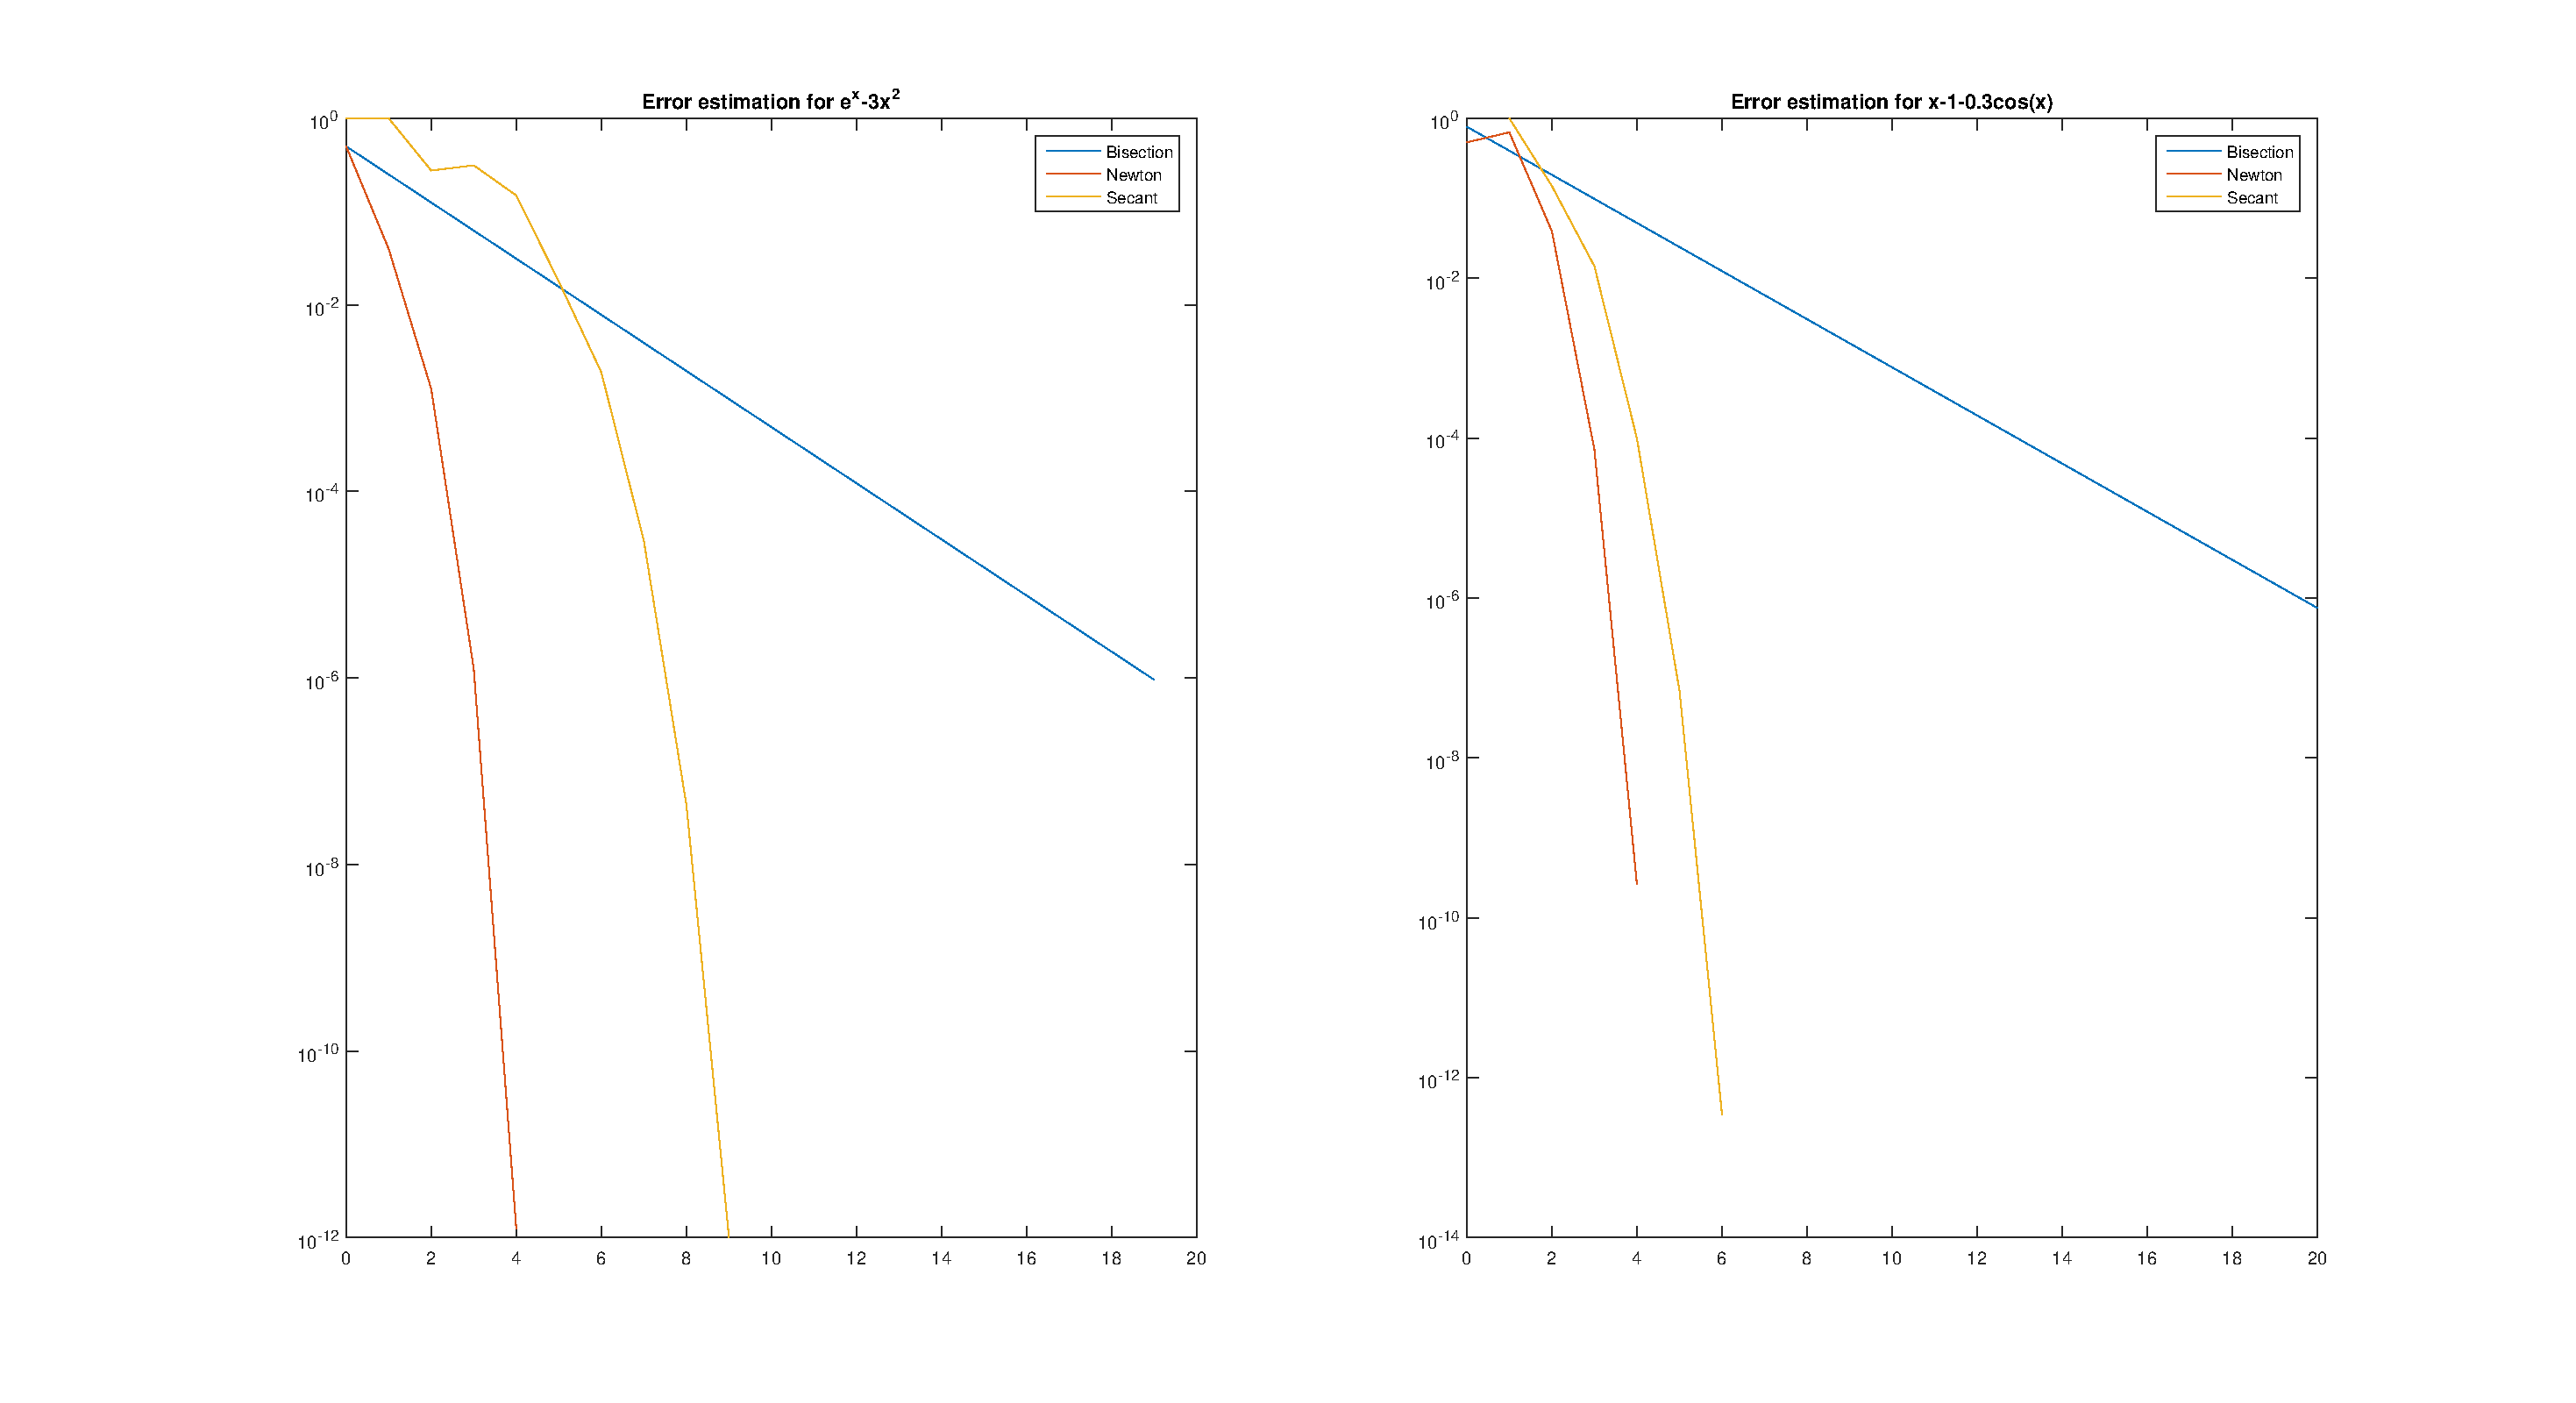
\includegraphics[width = 18cm]{res.eps}
\caption{Error Estimation}
\label{Figure 1}
\end{figure}

\problem{2}{Problem 2.12, Page 119}
\solution{Solution}{
Denote 
$$
f(x) = x^2-a,
$$
we know the Newton's scheme for this function is 
$$
x_{n+1} = x_n - \frac{f(x_n)}{f'(x_n)} = \frac{1}{2}(x_n + \frac{a}{x_n}).
$$
If we square both side of the equation, we can get
$$
x_{n+1}^2 - a = \left(\frac{x_n^2+a}{2x_n}\right)^2-a = \left(\frac{x_n^2-a}{2x_n}\right)^2.
$$
Then $x_n > \sqrt{a}$. Thus
$$
x_{n+1}-x_{n} = \frac{a-x_n^2}{2x_n} < 0,
$$
which means $\{x_n\}$ is a strictly decreasing sequence. If we consider the error, we can know
$$
e_{n+1} = \sqrt{a} - x_{n+1} = -\frac{(x_n-\sqrt{a})^2}{2x_n} = -\frac{e_n^2}{2x_n},
$$
and the relative error
$$
\text{Rel}(x_{n+1}) = \frac{e_{n+1}}{\sqrt{a}} = -\frac{e_n^2}{2\sqrt{a}x_n} = -\frac{\sqrt{a}}{2x_n}\left(\text{Rel}(x_n)\right)^2.
$$
Then
$$
|\text{Rel}(x_n)| = \left(\frac{\sqrt{a}}{2}\right)^n\frac{\text{Rel}(x_0)^{2^n}}{\prod_{i = 0}^{n-1}x_i} < \left(\frac{\sqrt{a}}{2}\right)^n\frac{\text{Rel}(x_0)^{2^n}}{(\sqrt{a})^n} = \frac{\text{Rel}(x_0)^{2^n}}{2^n}.
$$
Thus 
$$
|\text{Rel}(x_4)| < \frac{10^{-16}}{16}.
$$
}
\end{document}